% Chapter Template

\chapter{Analysis and Results - Passive Monitoring} % Main chapter title

\label{Chapter5} % Change X to a consecutive number; for referencing this chapter elsewhere, use \ref{ChapterX}

\lhead{Chapter 5. \emph{Analysis and Results - Passive Monitoring}} % Change X to a consecutive number; this is for the header on each page - perhaps a shortened title

\section{Analysis}
The final purpose of our system is to provide analysis about the main issues we have encountered in the wireless infrastructure. The way we process here is quite simple:

\begin{enumerate}
\item Put together the related information
\item Spot the anomalies
\item Try to understand the causes
\end{enumerate}
Like in any other system, we had to define domains on which the monitoring tool will be able to work. As a reminder, one of the first steps of this thesis was to determine what are or could be the main issues in the UCL's wireless network. This is typically on this step that we will use those results. Each of these problems will be represented by a domain in which we will define what the relevant data are, how they can help us, and how to correctly react after having analyzed them. 

The purpose of this chapter is to present these domains and the methodology we used to analyze them since they all have their particular needs and their related techniques of analysis.

\section{WiFi}

\subsection{Users}
This first section of the application offers some aggregated statistics about the users of the wireless network. The main objective is to get some analysis of the actual utilization of the wireless infrastructure. It is more like a set of indicators to help the administrators get a global and live overview of their network. 

\subsubsection*{WiFi Protocol}

The following graph displays the repartition of users among the available \texttt{802.11} standards (i.e. \texttt{802.11a, b, g, n}). 

\begin{figure}[H]
	\centering
   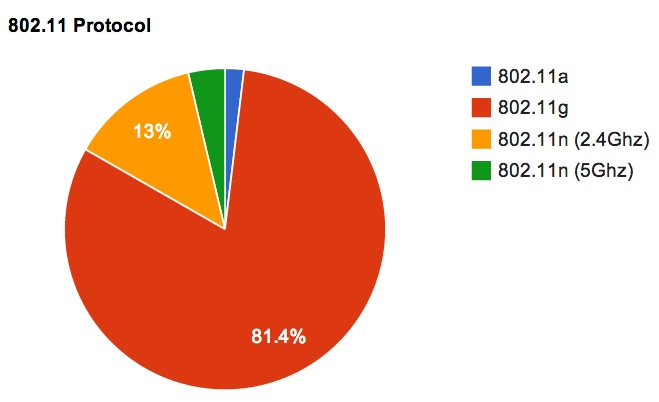
\includegraphics[width=0.6\textwidth]{Pictures/chapter5/ip-proto.jpg}
   \caption{Repartition of users among the \texttt{802.11} standards.}
\end{figure} 

The reason for this analysis comes from an earlier policy enforced on the UCL's network that forbids the use of the \texttt{802.11b} protocol. Users connecting with such low bandwidth standard force the access point to transmit longer and can, in consequence, prevent the others users to achieve higher receiving speed. This analysis was designed to help the administrators to have future information in the same domain. By profiling the habits of the users, we can define the impact of such decision. Since the quality of the service is one of the main concerns, deactivating the utilization of a standard used by most of the devices could have heavy consequences.

The statistics are based, by default, on the connection establishments made during the last three months. This to ensure that devices no longer connected to the network do not affect the results, and to keep the analysis as up-to-date as possible.

\paragraph*{Sources} The data used come from \texttt{SNMP} requests. During each cycle we gather information about all the devices associated with the access points thanks to the values available on the controller. All the descriptions of the \texttt{OIB} come from the \texttt{Cisco OID Browser}\footnote{http://tools.cisco.com/Support/SNMP/do/BrowseOID.do}.

\noindent
\begin{tabular}{|r l|}
\hline 
\textbf{Object} & \texttt{bsnMobileStationProtocol} \\
\textbf{Description} & \parbox{11cm}{The \texttt{802.11} protocol type of the client. The protocol is mobile when this client detail is seen on the anchor i.e. it is mobility status is anchor.} \\
\textbf{OID} & 1.3.6.1.4.1.14179.2.1.4.1.25 \\
\textbf{MIB} & AIRESPACE-WIRELESS-MIB \\
\hline
\end{tabular}

\subsubsection*{SSID Utilization}
Here, we count the number of users by \texttt{SSID}. As before, the goal is to provide a complete profile of the users to the administrators. Such measures can help them to adapt the policies related to each \texttt{VLAN} and defining the load of each of them. It could help to diagnostic a useless \texttt{VLAN} or in the opposite, it could allow to detect an overloaded one that might be caused by an improper use of the network. The supposed utilization and the actual one can be really different and such indicators can help the administrators to adapt the \texttt{VLAN} configurations. Here is the representation of the \texttt{SSID} utilization.
\begin{figure}[H]
	\centering
   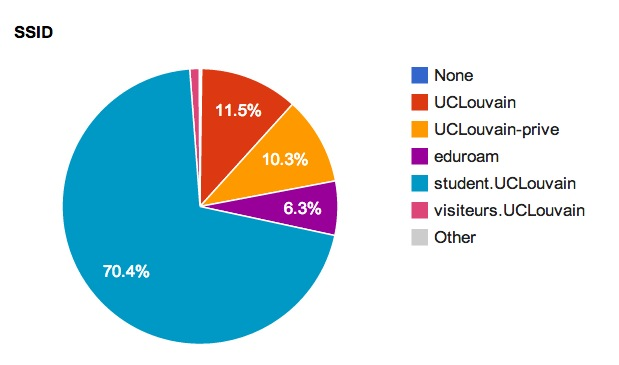
\includegraphics[width=0.7\textwidth]{Pictures/chapter5/ssid-utilization.jpg}
   \caption{\texttt{SSID} utilization}
\end{figure} 

\paragraph*{Source:} As before, we mainly aggregate the data available on the controller.

\begin{tabular}{|r l|}
\hline
\textbf{Object} & \texttt{bsnMobileStationSsid} \\
\textbf{Description} & \parbox{11cm}{The SSID Advertised by Mobile Station.} \\
\textbf{OID} & 1.3.6.1.4.1.14179.2.1.4.1.7 \\
\textbf{MIB} & AIRESPACE-WIRELESS-MIB \\
\hline
\end{tabular}

\subsection{Access Point}
This section regroups several analysis related to the \emph{access points}. In a network with several hundreds of access points, it can be difficult to diagnose and monitor each one of them. By centralizing and aggregating the data, we allow the network managers to save time by automatizing lot of computations. In this part of the application, we have access to the monitoring information of each access point currently associated with the controller.

\subsubsection*{Load}
A fundamental piece of information related to an access point is the load. We monitor each spot continuously and record its state several times per hour. By analyzing those data, we are able to plot graphs representing the load throughout the days. To do that, we need two information: the \textit{quantity} of data transiting on the link and the \textit{maximum speed} of that link. Concretely, each \texttt{AP} owns two byte counters that are incremented each time a byte is received or sent. The other information required is the link speed connecting the spot (this information on itself can be useful to diagnostic bandwidth issues). 

\paragraph*{Links} In a big network, it can be difficult to keep track of which links were updated and which ones were not. By collecting these data, we were able to find that two \emph{access points} were still connected with a \texttt{10 Mbits} link. For this case, the cause was that those concerned devices were not managed by the \texttt{SGSI} and in consequence were not upgraded with the others. Those APs are located in the \texttt{Stevin} building.
This is an example that even such simple data can help diagnostic some inconsistencies in the network.

\begin{figure}[H]
   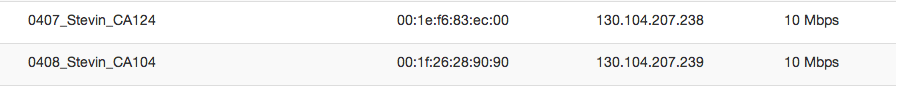
\includegraphics[width=\textwidth]{Pictures/chapter5/slowLinks.png}
   \caption{Example of 10Mbits Links (26/06/2014)}
\end{figure}

\paragraph*{Pattern of Utilization} By taking a look at the results, we can see during which periods of time the access point is the most active. In the example below, we have chosen an access point of the \texttt{Leclercq} building and displayed the results of several days of monitoring. As expected, almost no activity is detected during the night. It really starts around 9 am. 

\begin{figure}[H]
   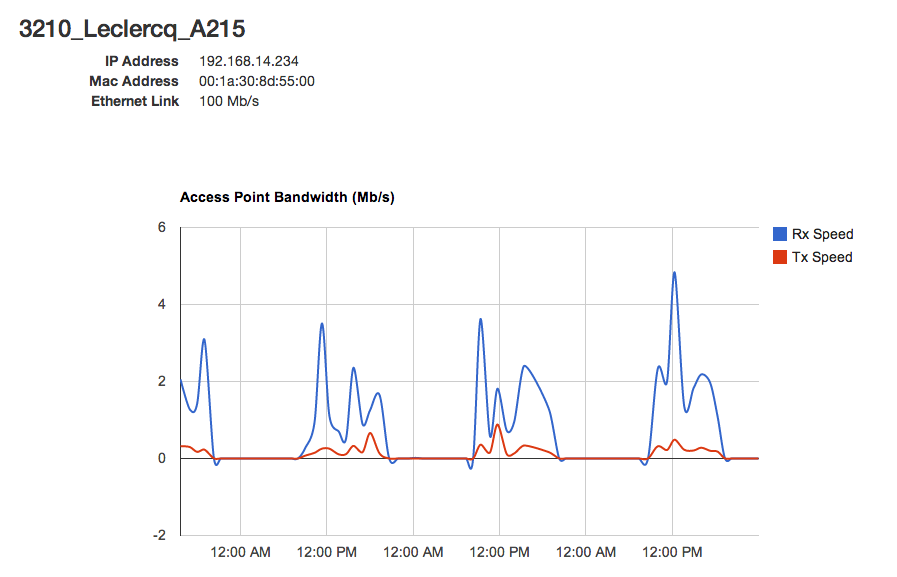
\includegraphics[width=\textwidth]{Pictures/chapter5/apLoad.png}
   \caption{Access Point Load}
\end{figure}

\paragraph*{Sources} Here again, we use the data available on the controller. The first data collected are the byte counters of each access point.

\begin{tabular}{|r l|}
\hline
\textbf{Object} & \texttt{cLApEthernetIfRxTotalBytes} \\
\textbf{Description} & \parbox{11cm}{This object represents the total number of bytes in the error-free packets received on the interface.} \\
\textbf{OID} & 1.3.6.1.4.1.9.9.513.1.2.2.1.13 \\
\textbf{MIB} & CISCO-LWAPP-AP-MIB \\
\hline
\end{tabular}

\begin{tabular}{|r l|}
\hline
\textbf{Object} & \texttt{cLApEthernetIfTxTotalBytes} \\
\textbf{Description} & \parbox{11cm}{This object represents the total number of bytes in the error-free packets transmitted on the interface.} \\
\textbf{OID} & 1.3.6.1.4.1.9.9.513.1.2.2.1.14 \\
\textbf{MIB} & CISCO-LWAPP-AP-MIB \\
\hline
\end{tabular}

The next step is to obtain the speed of each link connected to an access point. This time again we use the \texttt{SNMP} protocol to get the information from the controller.

\begin{tabular}{|r l|}
\hline
\textbf{Object} & \texttt{cLApEthernetIfLinkSpeed} \\
\textbf{Description} & \parbox{11cm}{Speed of the interface in units of 1,000,000 bits per second.} \\
\textbf{OID} & 1.3.6.1.4.1.9.9.513.1.2.2.1.11 \\
\textbf{MIB} & CISCO-LWAPP-AP-MIB \\
\hline
\end{tabular} 

\subsubsection*{Interfaces}
Each access point has two WiFi interfaces. The first one emits at \texttt{5Ghz} and the second at \texttt{2,4Ghz}. For each interface, the controller provides a lot of information that can be used in parallel of the previous ones. The first that we gather is the \textit{number of users} currently associated to the interface. We complete that information with the quantity of users with a poor \texttt{Signal-Noise Ratio} (SNR). This analysis allows to diagnostic the efficiency of the access point. Even if it may be considered normal to have a couple of users in this category, if the proportion is constantly high, it can be an indicator that a supplementary access point might be helpful, or that the location of the AP is problematic. The problems have to be put in perspective with the \texttt{RF} environment (i.e. \texttt{Rogue Access Points} or physical walls) which is outside the scope of this monitoring system. 
Finally, we complete this analysis with a monitoring of the \emph{channel utilization}. A high utilization of the channel results in poor connection quality for the user and could indicates weak \texttt{RF} conditions.
Here is a representation of a \texttt{2.4GHz} interface with information related to the client occupancy, the occupancy of client with a poor \texttt{SNR} and the channel utilization. 

\begin{figure}[H]
   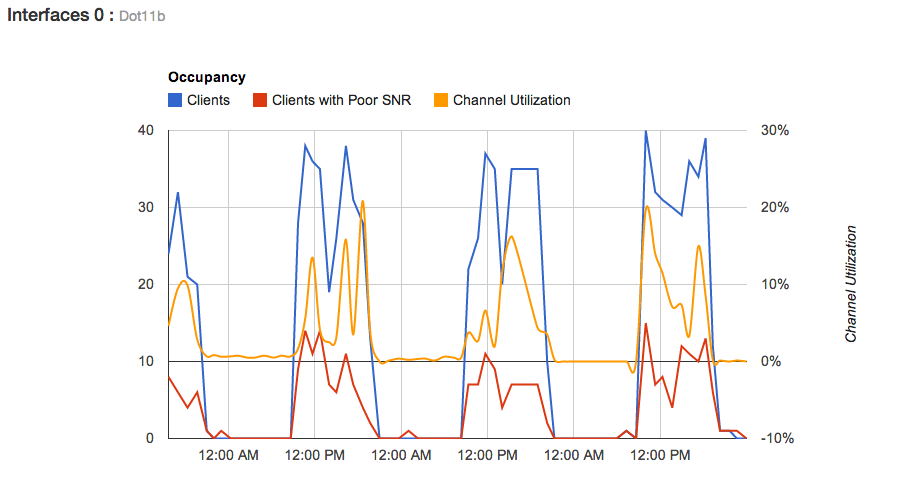
\includegraphics[width=\textwidth]{Pictures/chapter5/interfaceLoad.png}
   \caption{A 2,4GHz Interface}
\end{figure}

\paragraph*{Poor SNR} To illustrate our results, we have taken the 2,4GHz interface of the previous access point (i.e. \texttt{3210 Leclercq A215}) during the same period of time. As we can see, the load of the access point is correlated with the number of people connected to the interface. In this situation, we observe that there is an average of one-third or one-fourth of users with a poor SNR. This can be related to the configuration of the building. There is a large number of walls that separate the class room. The last thing to consider is the definition of a \emph{poor} \texttt{SNR}. This value is completely defined by the controller. In definitive, we do not have any access nor control on that parameter. Finally, in order to understand the importance of this result, we have to be aware that if a large portion of users has a low signal, it might influence the other devices with a good one. Indeed, the access points may have to spend more time sending data to those users with a low signal and, by consequence, are unavailable for others connections.

\paragraph*{Channel Utilization} The channel is a shared resource and need to be available in order to be used. The utilization of the channel is an important monitoring indicator. It allows the network administrators to estimate the quality of the users connections. If the medium is used at more than fifty percent, latency-sensitive applications can experience some performance issues \cite{ciscoVowlan}. A continuous monitoring of that value can help to detect and diagnostic such related problems. In our example, we can see that there is some maximum peaks at twenty percent of utilization which are totally acceptable. 


\paragraph*{Sources} The controller keeps entries for each \emph{interface} of each access point. We gather and cross all these data to generate some logs about each \emph{access point} and all the related \emph{interfaces}.

\begin{tabular}{|r l|}
\hline
\textbf{Object} & \texttt{bsnAPIfLoadNumOfClients} \\
\textbf{Description} & \parbox{11cm}{This is the number of clients attached to this Airespace AP at the last measurement interval.} \\
\textbf{OID} & 1.3.6.1.4.1.14179.2.2.13.1.4 \\
\textbf{MIB} & AIRESPACE-WIRELESS-MIB \\
\hline
\end{tabular}

\begin{tabular}{|r l|}
\hline
\textbf{Object} & \texttt{bsnAPIfPoorSNRClients} \\
\textbf{Description} & \parbox{11cm}{This is the number of clients with poor SNR attached to this Airespace AP at the last measurement interval.} \\
\textbf{OID} & 1.3.6.1.4.1.14179.2.2.13.1.24 \\
\textbf{MIB} & AIRESPACE-WIRELESS-MIB \\
\hline
\end{tabular}

\begin{tabular}{|r l|}
\hline
\textbf{Object} & \texttt{bsnAPIfLoadChannelUtilization} \\
\textbf{Description} & \parbox{11cm}{Channel Utilization.} \\
\textbf{OID} & 1.3.6.1.4.1.14179.2.2.13.1.3 \\
\textbf{MIB} & AIRESPACE-WIRELESS-MIB \\
\hline
\end{tabular}

\subsection{Rogue Access Points}
For the \texttt{rogue access points}, we chose to group them by their estimated position. For each one of them, we know what is the closest AP that detects it. From that information we can tell where they are and we can generate aggregated information about the areas that contain the more rogue access points that we present on a graph. Here is an example of such representation.

\begin{figure}[H]
   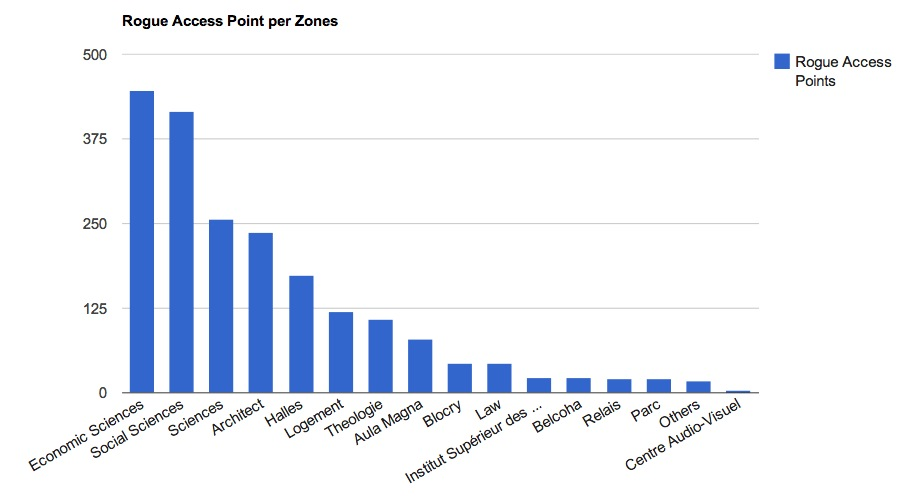
\includegraphics[width=\textwidth]{Pictures/chapter5/rogue-ap.jpg}
   \caption{Number of Rogue AP by area}
\end{figure}


\section{Controller}
The controller logs are divided in several categories. Each of them defines a list of logs related to that category. The main idea here is to analyze the activity of each domain of logs and trying to spot irregularities. We make the hypothesis that when something goes wrong, the related category will emit a larger number of logs. By monitoring that activity, we will be able to identify in which part of the infrastructure the issue happened. More powerful analysis could be easily implemented but that would require to target some specific syslogs. That could be really useful if the administrators want to monitor specific events and detect certain patterns. But that is only relevant to detect very precise elements and we have chosen to focus on a more global monitoring system.

\subsection{Components Activity}
The idea here is to have a representation of the logs generated by each component throughout the day. With such representation, we can detect some peak of activity that could indicate an issue.


\section{DHCP}
These analyses aim to detect \texttt{DHCP} related issues. The allocation of IP addresses is a fundamental component in the wireless networks. Being able to detect when such problem appears and advertise them directly in our application might help making a quicker and more efficient response.

\subsection{Leases}
The main challenge with a \texttt{DHCP} server is the configuration of the address ranges. It is always difficult to determine the quantity of IP addresses the \texttt{VLANs} require. If no more \texttt{IP} address is available for a user he won't be able to access the Internet despite the fact that he has established a connection with the AP. The main issue is that when such problem arises it can be hard to be aware of them. Indeed, most of the time the users do not report the problem to the network administrators or if they do, their explanations of the problem are not very precise, complicating the tasks of those administrators. Being able to automatically detect the lack of \texttt{IP} addresses can thus be very time saving. Even if those information are available within the \texttt{DHCP} logs and that those servers can send warnings in case of trouble, centralizing them and aggregating them with data related to all the other network components may lead to more powerful analysis.

\paragraph*{Misleading Error Messages} When we started to investigate on this issue, we tried to find what kind of logs the \texttt{DHCP} servers had generated in such circumstances. The answer is that the servers simply indicate that situation by adding \texttt{peer holds all free leases} next to the \texttt{Discover} log. So, we have searched for such messages in the log files and we have found some of them among other normal \texttt{Discover} messages. It seems odd that if no lease is available for someone, it is for the others. That might be explained by the fact that the users are not connected in the same \texttt{VLAN}. But what really bothered us is the fact that only specific devices are concerned by this error message. Each time one of those device sends its \texttt{Discover} message, the two \texttt{DHCP} servers responds with the \texttt{peer holds all free leases} message. We have created an analysis mechanism to recognize that error pattern and to list the potential affected devices. \\

\begin{lstlisting}[frame=single,breaklines=true,caption={Misleading Error Message}]
2014-05-28T13:03:02.628508+02:00 dhcp-1 dhcpd: DHCPDISCOVER from AB:CD:EF:12:34:56 via 130.104.238.254: peer holds all free leases
2014-05-28T13:03:02.628553+02:00 dhcp-2 dhcpd: DHCPDISCOVER from AB:CD:EF:12:34:56 via 130.104.238.254: peer holds all free leases
\end{lstlisting}


The next step of our investigation was to find what could be the source of that error pattern. We found an interesting answer on an online post from a network administrator\footnote{http://noone.org/blog/English/Computer/peer\%20holds\%20all\%20free\%20leases.html}. He explains that if we observe such messages from the two server at the same time, the cause could be a device connected on a wrong \texttt{VLAN}. If the \texttt{VLAN} is configured to only distribute static \texttt{IP}, the device asking for a dynamic one would be unable to obtain it. The main difficulty here is to make the difference between this situation and the one in which there is no more \texttt{IP} addresses available.


\paragraph*{No more lease} Most of the time, the ranges of \texttt{IP} addresses are large enough and the previous hypothesis about the \texttt{no free lease} messages holds. But how could we detect a real issue concerning the \texttt{IP} range ? To enhanced the previous results, we have added an indicator of the current \texttt{DHCP} server state. We compute the ratio of the number of error messages to the quantity of affected devices. The smaller the result, the more chances the \texttt{DHCP} has an actual \texttt{IP} range issue. We call this ratio the \emph{scatter degree} of the lease issue. Notice that, if the problem is concentrated on a small set of devices, there are a lot of chances that the source is not the \texttt{DHCP} but is the Ethernet sockets being used.
\[ \frac{Nbr\ of\ \texttt{no free lease}\ messages}{Nbr\ of\ affected\ devices} \] 


\subsection{Crash}
Another issue we have been able to monitor was the crash of the \texttt{DHCP} servers on the 4$^{th}$ of March 2014. As we can see on the figure below that represents only a 15 minutes sample of the \texttt{DHCP} log file, there was an important number of \texttt{Discover} packets without any \texttt{Offer} packets in return. With such a representation, we are able to locate more precisely where the network problem came from. Because the servers were not even able to send any \texttt{Offer} packets, we had easily made the hypothesis that the entire \texttt{DHCP} servers were down.

\begin{figure}[H]
	\centering
   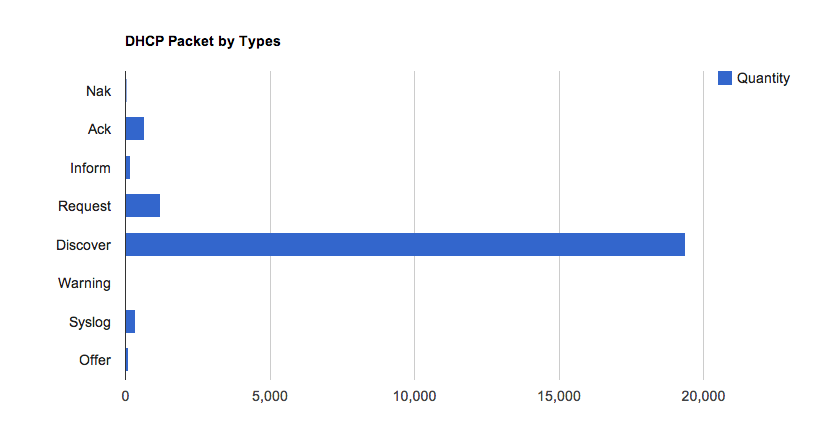
\includegraphics[width=1\textwidth]{Pictures/chapter5/dhcpCrash.png}
   \caption{DHCP Crash - 04/04/14}
\end{figure}

\section{RADIUS}
The analysis we made about the \texttt{RADIUS} are quite limited by the verbosity of the logs and by the fact that we do not have any access to the server. What we have chosen to monitor here are some general indicators.

\subsection{Authentication Success Rate}
The first thing we can observe about the \texttt{RADIUS} is the proportion of users being able to authenticate. If this rate drastically drops, that could indicate issues about the \texttt{RADIUS} server. This indicator alone does not bring much information but could be compared with the average authentication success rate to detect some important divergences.

\paragraph*{Overall Success Rate} The purpose of this graph is to get an idea of the average authentication success rate. Concretely, it counts the logs showing the messages \textit{login success} or \textit{fail}. Here again, we do not keep data about specific users. All the data are aggregated to compute the desired ratio. Each of these logs contains sensible information about the user and the time at which he established a connection with an AP. By crossing this information with the access point, we may follow his position throughout the day. We chose to limit this possibility by not linking those information together in the database. Even if this limitation could be easily broken, it's more an ethical consideration than a security issue.

\begin{figure}[H]
	\centering
   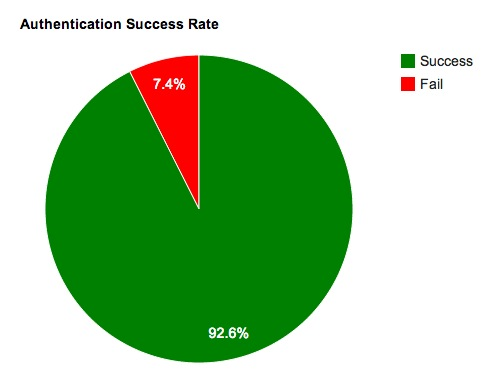
\includegraphics[width=0.5\textwidth]{Pictures/chapter5/radiusRate.jpg}
   \caption{Example of \texttt{RADIUS} Success Rate}
\end{figure} 

\paragraph*{Sources} The sources of those data are the \texttt{RADIUS} log files. These files contains an entry for each authentication attempt. Here is an example of the success and fail message we find in the \texttt{RADIUS} log files.
\begin{lstlisting}[frame=single,breaklines=true,caption={\texttt{RADIUS} logs}]
2013-10-21T17:27:48+02:00 radius1.sri.ucl.ac.be radiusd[17913]: [ID 702911 local4.notice] Login incorrect: [XXXX] (from client WiSMPythagore-A port 29 cli XX-XX-XX-XX-XX-XX)
2013-10-21T17:27:50+02:00 radius1.sri.ucl.ac.be radiusd[17913]: [ID 702911 local4.notice] Login incorrect: [none] (from client WiSMPythagore-A port 29 cli XX-XX-XX-XX-XX-XX)
2013-10-21T17:27:55+02:00 radius1.sri.ucl.ac.be radiusd[1523]: [ID 702911 local3.notice] Login OK: [XXXX] (from client WiSMStevin-B port 29 cli XX-XX-XX-XX-XX-XX)
2013-10-21T17:27:55+02:00 radius1.sri.ucl.ac.be radiusd[1523]: [ID 702911 local3.notice] Login OK: [XXXX] (from client localhost port 0)
2013-10-21T17:27:59+02:00 radius1.sri.ucl.ac.be radiusd[1523]: [ID 702911 local3.notice] Login OK: [XXXX] (from client WiSMStevin-B port 29 cli XX-XX-XX-XX-XX-XX)
\end{lstlisting}

\section{Summary}
This chapter detailed the main results developed by our application from the data gathered with the \texttt{SNMP} protocol and the several log files. The main interest of gathering these data comes from the fact that they are linked together. Notice that all the data are already available on the controller but by trying to correlate some of them, we wanted to give another view of the network and shed light on some misunderstood issues. 

